\documentclass[main.tex]{subfiles}
\begin{document}

\chapter{Funktionsuntersuchung}\label{Funktionsuntersuchung}
\chapterauthor{Bruno}

Die \textbf{Analysis} (griechisch  análysis, deutsch "`Auflösung"') ist ein Teilgebiet der Mathematik. Die Untersuchung von reellen und komplexen Funktionen hinsichtlich Stetigkeit, Differenzierbarkeit und Integrierbarkeit zählt zu den Hauptgegenständen der Analysis. Die hierzu entwickelten Methoden sind in allen Natur- und Ingenieurwissenschaften von großer Bedeutung.

\section{Stetigkeit}

\begin{Definition}
	Eine Funktion ist stetig an der Stelle $x_{0}$, wenn:
	\begin{enumerate}
		\item $x_{0}\in D$
		\item $\lim\limits_{x \rightarrow x_{0}} {f(x)}$ existiert
		\item $\lim\limits_{x \rightarrow x_{0}^{\pm}} {f(x)}=f(x_{0})$
	\end{enumerate}
\end{Definition}

Stetigkeit ist eine lokale Eigenschaft. Die Funktion $f$ heißt dann stetig, wenn sie an jeder Stelle ihrer Definitionsmenge stetig ist.

\begin{Bemerkung}
	\begin{Theorem}
		Ist $f$ stetig und $I\subset \R$ ein reelles Intevall, dann ist $f(I)$ ebenfalls ein Intervall. Ist $f$ zudem streng monoton, so ist die Umkehrfunktion $f^{-1}$ ebenfalls stetig.
	\end{Theorem}
\end{Bemerkung}

\begin{Bemerkung}
	Stetige Funktionen haben sehr angenehme Eigenschaften, die intuitiv mit der ''Definition'' des Stiftes, welcher beim Zeichnen des Funktionsgraphen nicht angehoben wird, im Zusammenhang stehen.
	
	So sagt der \textbf{Zwischenwertsatz} aus, dass eine reelle, im Intervall $[a;b]$ stetige Funktion $f$ jeden Wert zwischen $f(a)$ und $f(b)$ ainnimmt.

	Haben $a$ und $b$ zudem verschiedene Vorzeichen, so verspricht der Zwischenwertsatz mindestens eine Nullstelle von $f$ in diesem abgeschlossenen Intervall. Dieser Sonderfall ist als \textbf{Nullstellensatz} von Bolzano bekannt.
\end{Bemerkung}

\begin{Theorem}[Zwischenwertsatz]
	Ist $f:[a;b]\Rightarrow$ eine stetige reelle Funktion die auf einem Intervall definiert ist, dann existiert zu \textbf{jedem} $s \in [f(a);f(b)]$ bzw. $[f(b);f(a)]$ (vom Vorzeichen der Funktionswerte abhängig) \textbf{ein} $c \in [a;b] $ mit $f(c)=s$
\end{Theorem}


\subsubsection{Stetige Fortsetzungen}

Beim Vereinfachen von gebrochenrationalen Funktionen ist Vorsicht geboten, denn eine hebbare Definitionslücke ''aufzuheben'' verändert den Definitionsbereich der Funktion. Die daraus resultierende Funktion wird \textbf{stetige Fortsetzung} genannt.



\section{Differenzierbarkeit}

\begin{Definition}
	Eine Funktion ist differenzierbar an der Stelle $x_{0} \in D$, wenn der beitseitige Grenzwert des Differenzenquotienten für $h\rightarrow 0$ existiert. Anschaulich soll Die Funktion links und rechts des $x_{0}$ die selbe Ableitung haben.

	$\lim\limits_{h \rightarrow 0^{+}} {\dfrac{f(x_{0}+h)-f(x_{0})}{h}} = \lim\limits_{h \rightarrow 0^{-}} {\dfrac{f(x_{0}+h)-f(x_{0})}{h}} =f'(x_{0})$

	Dieser Grenzwert ist die \textbf{Ableitung} von $f$ an der Stelle $x_{0}$.

	Die Funktion heißt differenzierbar, wenn sie $\forall x \in D$ differenzierbar ist.
\end{Definition}


Die Funktion $f(x)=|x|$ ist nicht differenzierbar, da bei der Stelle $x_{0}=0$ der linksseitige Grenzwert des Differenzenquotienten ($\lim\limits_{h \rightarrow 0^{-}}{f'(x_{0})=-1}$) nicht mit dem rechtsseitigen Grenzwert (1) übereinstimmt.


\subsection{Zusammenhang zwischen Stetigkeit und Differenzierbarkeit}

Ist eine Funktion $f$ an der Stelle $x_{0}$ differenzierbar, so ist sie an dieser Stelle auch stetig.

Die Umkehrung gilt erst einmal nicht, aber es gibt eine verneinende Aussage: Ist $f$ an der Stelle $x_{0}$ nicht stetig, so ist sie hier auch nicht differenzierbar.

\begin{Theorem}
	$f$ differenzierbar $\Rightarrow f$ stetig.
\end{Theorem}
\begin{Bemerkung}
	Ist eine Funktion differenzierbar und ist ihre Ableitung zusätzlich stetig, dann wird sie \textbf{Stetig differenzierbar} genannt.
\end{Bemerkung}


\section{Ableitungsregeln}

Ein Ableitungswert gibt die Steigung an einem bestimmten Punkt an. Im Allgemeinen und zum Beweisen wird der Differentenquotient benötigt, um eine Ableitungsfunktion zu definieren, es geht aber in vielen Fällen schneller.

\begin{Theorem}[Produktregel]
	Sind die Funktionen $u$ und $v$ an der Stelle $x_{0}$ $\in$ $D$ differenzierbar, dann ist die Funktion $f(x)=u(x)\cdot v(x)$ bei $x_{0}$ auch differenzierbar und es gilt:
	$$f'(x_{0}) = u'(x_{0})v(x_{0})+u(x_{0})v'(x_{0})$$
\end{Theorem}

\begin{Beweis}
	$$\begin{array}{rcl}
		\lim\limits_{h \rightarrow 0} {\dfrac{f(x_{0}+h)-f(x_{0})}{h}} & = & \lim\limits_{h \rightarrow 0} {\dfrac{u(x_{0})v({x_{0}+h)-u(x_{0})v(x_{0})}}{h}}\\
		&=&\lim\limits_{h \rightarrow 0} {\dfrac{u(x_{0}+h)v(x_{0}+h)\textcolor{red}{-u(x_{0})v(x_{0}+h)+u(x_{0})v(x_{0}+h)}-u(x_{0})v(x_{0}) }{h}}\\
		&=&\lim\limits_{h \rightarrow 0} {\dfrac{u(x_{0}+h)v(x_{0}+h)-u(x_{0})v(x_{0}+h)}{h}} + \lim\limits_{h \rightarrow 0} {\dfrac{u(x_{0})v(x_{0}+h)-u(x_{0})v(x_{0})}{h}}\\
		&=&\lim\limits_{h \rightarrow 0} {v(x_{0}+h)\dfrac{u(x_{0}+h)-u(x_{0})}{h}} \lim\limits_{h \rightarrow 0} {u(x_{0})\dfrac{v(x_{0}+h)-v(x_{0})}{h}}\\
		&=& v(x_{0})\lim\limits_{h \rightarrow 0}{\dfrac{u(x_{0}+h)-u(x_{0})}{h}} +u(x_{0}) \lim\limits_{h \rightarrow 0} {\dfrac{v(x_{0}+h)-v(x_{0})}{h}}\\
		&=& u'(x_{0})v(x_{0}) - u(x_{0})v'(x_{0})
	\end{array}$$
\end{Beweis}

\begin{Theorem}[Quotientenregel]
	Sind die Funktionen $u$ und $v$ an der Stelle $x_{0}$ $\in$ $D$ differenzierbar, dann ist die Funktion $f(x)=\frac{u(x)} {v(x)}$ bei $x_{0}$ auch differenzierbar und es gilt:

	$$f'(x_{0})=\frac{u'(x_{0})\cdot v(x_{0})-u(x_{0})\cdot v'(x_{0})}{v^2(x_{0})}$$
\end{Theorem}

\begin{Beweis}
	$$\begin{array}{rcl}
		\lim\limits_{h \rightarrow 0} {\dfrac{f(x_{0}+h)-f(x_{0})}{h}}&=& \lim\limits_{h \rightarrow 0} { \dfrac{ \dfrac{u(x_{0}+h)} {v(x_{0}+h)}- \dfrac{u(x_{0})}  {v(x_{0})}}  {h}}\\
		&=&\lim\limits_{h \rightarrow 0} {\dfrac{\dfrac {u(x_{0}+h)}{v(x_{0}+h)}-\dfrac {u(x_{0})} {v(x_{0})}}   {h}}\\
		&=&\lim\limits_{h \rightarrow 0} {\dfrac {\dfrac{  u(x_{0}+h)v(x_{0})}{v(x_{0}+h)v(x_{0})}   -\dfrac{u(x_{0})v(x_{0}+h)}{v(x_{0})v(x_{0}+h))}} {h}}\\
		&=&\lim\limits_{h \rightarrow 0} {\dfrac     {u(x_{0}+h)v(x_{0})-u(x_{0})v(x_{0}+h)}    {v(x_{0}+h)v(x_{0})h }}\\
		&=&\lim\limits_{h \rightarrow 0} {\dfrac {u(x_{0}+h)v(x_{0}) \textcolor{red}{-u(x_{0})v(x_{0})} -u(x_{0})v(x_{0}+h) \textcolor{red}{+u(x_{0})v(x_{0})}}  {v(x_{0}+h)v(x_{0})h}   }\\
		&=&\lim\limits_{h \rightarrow 0} {\dfrac   {\dfrac{u(x_{0}+h)v(x_{0})-u(x_{0})v(x_{0})}{h}  -   \dfrac{u(x_{0})v(x_{0}+h)-u(x_{0})v(x_{0})} {h} }    {v(x_{0}+h)v(x_{0})}}\\
		&=&\lim\limits_{h \rightarrow 0} { \dfrac     {\dfrac{u(x_{0}+h)-u(x_{0})}{h} v(x_{0})  -   u(x_{0}) \dfrac   {v(x_{0}+h)-v(x_{0})}  {h}  }         {v(x_{0}+h)v(x_{0})}     }\\
		&=&\lim\limits_{h \rightarrow 0} { \dfrac  {\lim\limits_{h \rightarrow 0} {\dfrac{u(x_{0}+h)-u(x_{0})}{h}   }v(x_{0})  - u(x_{0}) \lim\limits_{h \rightarrow 0} { \dfrac{ v(x_{0}+h)-v(x_{0})}{h}   }  }      {v(x_{0})v(x_{0})}}    \\
		&=& { \dfrac{u'(x_{0})v(x_{0})-u(x_{0})v'(x_{0})} {(v(x_{0}))^2}}
	\end{array}$$
\end{Beweis}

\begin{Theorem}[Kettenregel]
	 Funktion $v$ sei an der Stelle $x_{0}$ differenzierbar und die Funktion $u$ an der Stelle $v(x_{0})$. Dann ist die Funktion $f=u\circ v$ mit der Gleichung $f(x)= u(v(x))$ an der Stelle $x_{0}$ differenzierbar. Es gilt:
	$$f'(x_{0})=v'(x_{0})\cdot u'(v(x_{0}))$$
\end{Theorem}


\subsection{Tangente und Normale}

\begin{Theorem}
	Ist die Funktion $f$ differenzierbar an der Stelle $x_{0}$, dann hat die \textbf{Tangente} an dem Graphen von $f$ die Steigung $a=f'(x_{0})$ und den Y-Achsenabschnitt $b=-f'(x_{0})\cdot x_{0}+f(x_{0})$. Daraus ergibt sich die Tangentengleichung:
	$$T_{x_{0}}(x)=f'(x_{0})\cdot (x-x_{0})+f(x_{0}) $$
\end{Theorem}

\begin{Bemerkung}
	Eine Merkhilfe dazu ist das Wort "`Fuxufu"', wobei "`u"' dem $x_{0}$ entspricht.
\end{Bemerkung}

\begin{Definition}
	Die \textbf{Normale} an der Stelle $x_{0}$ bezeichnet die Gerade, die genau senkrecht zur Tangente steht und diese im Berührpunkt des Graphen schneidet.
	$$N_{x_{0}}(x)=-\frac{1}{f'(x_{0})}\cdot (x-x_{0})+f(x_{0})$$
\end{Definition}


\section{Vollständige Funktionsuntersuchung}


\subsection{Definitionsbereich}

Am Anfang muss der Definitionsbereich angegeben werden, um eventuelle Divisionen durch null zu vermeiden. Man achte dabei auch auf hebbare Definitionslücken (siehe ''Stetigkeit'')


\subsection{Achsenschnittpunkte}

Es gibt zwei Arten von Achsenschnittpunkten:
\begin{enumerate}
	\item X-Achsenschittpunkte (Nullstellen), die man mit der notwendigen und hinreichenden Bedingung für Nullstellen $f(x)=0$ herausfindet
	\item Y-Achsenschnittpunkt, den man durch einsetzen bekommt: $f(0)$
\end{enumerate}

\subsection{Symmetrie}

\subsubsection{Y-Achsensymmetrie}

Durch Lösung der Gleichung $f(x)=f(-x)$ findet man heraus ob die Funktion achsensymmetrisch ist.

Zudem ist die Funktion dann achsensymmetrisch, wenn nur gerade Exponenten vorhanden sind.

Die Funktion nennt man \textbf{gerade}.


\subsubsection{Symmetrie zum Origo}

Durch Lösung der Gleichung $f(x)=-f(-x)$ findet man heraus ob die Funktion punktsymmetrisch ist.

Zudem ist die Funktion dann punktsymmetrisch, wenn nur ungerade Exponenten vorhanden sind.

Die Funktion nennt man \textbf{ungerade}.


\subsubsection{Symmetrie zu einem beliebigen Punkt}

\begin{Definition}
	Symmetrie zu einem Punkt liegt vor, wenn für den Punkt $P(x_{0}|y_{0})$ gilt:
	$$f(x_{0}+h)-y_{0}=-f(x_{0}-h)+y_{0}$$
\end{Definition}

\begin{Beispiel}
	$f(x)=\frac{x}{x-1}$
	
	Aus dem Schnittpunkt der Asymptoten kann man vermuten, dass $f(x)$ achsensymmetrisch zum Punkt $P(1|1)$ ist.
	
	$\left. \begin{array}{rcl}
		\Rightarrow f(x_{0}+h)-y_{0}=\frac{1+h}{1+h-1}-1=\frac{1}{h}\\
		\Rightarrow -f(x_{0}-h)+y_{0}=-[\frac{1-h}{1-h-1}+1]=\frac{1}{h}
	\end{array} \right\} \frac{1}{h}=\frac{1}{h}$ Die Funktion $f$ ist zu $P$ symmetrisch.
\end{Beispiel}


\subsection{Grenzwerte}

\begin{Definition}
	Das Symbol $\lim\limits_{x \rightarrow x_{0}}f(x)$ mit $x_{0} \in \overline{\R}$ ($\pm \infty$ eingeschlossen) bezeichnet den Limes der reellen Funktion $f:D\rightarrow \R$ für den Grenzübergang von $x$ gegen eine Stelle $x_{0}$, wobei $x_{0}$ nicht umbedingt in der Definitionsmenge von $f$ enthalten sein muss.

	Eine Zahl $g \in \overline{\R}$ ist der Grenzwert einer Funktion $f:D\rightarrow \R$ für $x\rightarrow x_{0}$, falls für jede Folge $(a_{n})_{n\in \N}$ mit Folgegliedern aus $D$ und Grenzwert $x_{0}$ die Folge $(f(a_{n}))_{n\in \N}$ den Grenzwert $g$ hat.
	$$\lim\limits_{x \rightarrow x_{0}}f(x) = g \quad \Leftrightarrow \quad \forall (a_{n})_{n\in \N} \text{ mit } \lim\limits_{n \rightarrow \infty}a_{n}=x_{0} : \lim\limits_{n \rightarrow \infty}f(a_{n})=g$$
\end{Definition}

\begin{Theorem}[Règle de l'Hôpital (Für Grenzwerte des Typs $0/0$ und $\infty/\infty$)]
	Seien zwei differenzierbare Funktionen $f$ und $g$ und gelte entweder
	$$\lim\limits_{x \rightarrow x_{0}}g(x) = \lim\limits_{x \rightarrow x_{0}}f(x) = \infty \qquad \text{ODER} \qquad  \lim\limits_{x \rightarrow x_{0}}g(x) = \lim\limits_{x \rightarrow x_{0}}f(x) = 0$$
	(sie sind also entweder konvergent gegen $0$ oder bestimmt divergent) dann gilt:
	$$\lim\limits_{x \rightarrow x_{0}} \dfrac{f(x)}{g(x)} = \lim\limits_{x \rightarrow x_{0}}\dfrac{f'(x)}{g'(x)}$$
\end{Theorem}

\begin{Bemerkung}
	\begin{enumerate}
		\item Falls die Funktionsvorschrift nicht direkt ein Bruch ist (siehe 2. Beispiel) sollte man diese erst zu einem Bruch umformen, um mit der Hospital-Regel fortfahren zu können.
		\item ACHTUNG: Die Hospital-Regel ist nicht umkehrbar!
	\end{enumerate}
\end{Bemerkung}

\begin{Beispiel}
	$f(x) = \dfrac{\sin(x)}{x} \qquad x_{0} = 0\qquad \qquad D=\R\backslash\{0\}$

	$\Rightarrow \lim\limits_{x \rightarrow x_{0}}f(x) = \lim\limits_{x \rightarrow x_{0}}\dfrac{\sin(x)}{x} = \lim\limits_{x \rightarrow x_{0}} \dfrac{\cos(x)}{1} = 1 $

	$g(x) = x\cdot \log \left( \dfrac{x+1}{x-1} \right) \qquad $für $ x\to \infty \qquad \qquad D=\R\backslash\{1\}$

	$\begin{array}{rcl}
		\Rightarrow \lim\limits_{x \to \infty} g(x) & = & \lim\limits_{x \to \infty} x\cdot \log \left( \dfrac{x+1}{x-1} \right) \\
		&=& \lim\limits_{x \to \infty} \dfrac{\log \left( \dfrac{x+1}{x-1} \right) }{\dfrac{1}{x}}\\
		&=& \lim\limits_{x \to \infty} \dfrac{\dfrac{x-1}{x+1} \cdot \dfrac{-2}{(x-1)^2}}{-\dfrac{1}{x^2}}\\
		&=& \lim\limits_{x \to \infty} \dfrac{\dfrac{-2}{x^2-1}}{-\dfrac{1}{x^2}}\\
		&=& \lim\limits_{x \to \infty} \dfrac{2x^2}{x^2-1} = 2 \\
	\end{array}$
\end{Beispiel}


\subsection{Asymptoten}

Eine Asymptote ist eine Gerade oder Kurve, die sich dem Graphen einer Funktion immer weiter annähert. Dabei unterscheidet man verschiedene Fälle:

\begin{Definition}
	\begin{enumerate}
		\item \textbf{Senkrechte Asymptote:}
		
		Hat $f$ an der stelle $x_{0}$ eine Polstelle, und gilt:
			$$\lim\limits_{x \rightarrow x_{0^{\pm}}} f(x) = \pm \infty$$
		dann ist die Gerade $x=x_{0}$ eine senkrechte Asymptote von $f$.

		\item \textbf{Waagerechte Asymptote:}
		
		Konvergiert $f$ für $x\rightarrow \infty$ gegen eine reelle Zahl $g\in \R$, das heißt $\lim\limits_{x \rightarrow \infty }{f(x)}=g$, dann ist die Gerade $y=g$ die \textbf{waagerechte} Asymptote von $f$. Das Gleiche gilt für $\lim\limits_{x \rightarrow -\infty}$.\\
		Bei gebrochenrationalen Funktionen ist dies der Fall, wenn der Zählergrad kleiner (dann ist $g=0$) oder gleich dem Nennergrad $m$ ist.

		\item \textbf{Schräge Asymptote:}
		
		Sie ist eine Gerade ($g:\R \rightarrow \R$), der sich $f$ mit $|x|\rightarrow \infty$ beliebig annähert:
		$$\lim\limits_{x \rightarrow \infty}{[f(x)-g(x)]}=0 \text{ oder } \lim\limits_{x \rightarrow -\infty}{[f(x)-g(x)]}=0$$
		Bei einer gebrochenrationalen Funktion ist der ''Fehlergrad'', das heißt der Abstand von $g$ zu $f$ durch den Rest der Polynomdivision von Zähler mit Nenner gegeben.

		\item \textbf{Asymptotische Kurven:}
		
		Indem man in der Definition der schrägen Asymptote auch Polynome zulässt, erhält man Näherungskuven, die die gleiche Limesbedingung erfüllen müssen:
		$$\lim\limits_{x \rightarrow \infty}{[f(x)-P(x)]}=0 \text{ oder } \lim\limits_{x \rightarrow -\infty}{[f(x)-P(x)]}=0$$
		Diese erscheinen bei gebrochenrationalen Funktion mit $n>m+1$.
	\end{enumerate}
\end{Definition}

\subsection{Monotonie}

\begin{Definition}
	Eine stetige Funktion $f$ mit $a,b\in I \subset D_{f}$ ist:

	\begin{enumerate}
		\item ... auf dem Intervall $I$ monoton wachsend, wenn $\forall a < b: f(a)\leq f(b)$
		\item ... auf dem Intervall $I$ monoton fallend, wenn $\forall a < b: f(a) \geq f(b)$
	\end{enumerate}
	Wenn die Ordnungsrelation strikt sind, dann wird die Funktion als \textbf{streng monoton} bezeichnet.
	
	Die Funktion $f$ hat eine Ableitungsfunktion $f'$. Falls $f$...
	\begin{enumerate}
		\item monoton wachsend auf $I$ ist, dann ist $f'(x)\geq0$, \quad $\forall x \in I$
		\item monoton fallend auf $I$ ist, dann ist $f'(x)\leq0$, \quad $\forall x \in I$
		\item konstant auf $I$ ist, dann ist $f'(x)=0$, \quad $\forall x \in I$
	\end{enumerate}
	Beim Aufstellen der Monotonietabelle sind Definitionslücken zu beachten.
	
	Es handelt sich dabei um eine Tabelle, die die Definitionsmenge in Intervalle mit monotonen Steigungsverhalten unterteilt wird. Das Monotonieverhalten verändert sich an Extrem- oder Polstellen.
\end{Definition}

\begin{Bemerkung}
	$f$ sei eine Funktion...
	\begin{description}
		\item[$\bullet$] dann ist die Zahl $S$ obere Schranke, wenn $\forall x : f(x)\leq S$. $f$ heißt in diesem Fall nach oben beschränkt. Die in diesem Fall kleinstmögliche Zahl wird \textbf{Supremum} genannt: sup$f$
		\item[$\bullet$] dann ist die Zahl $s$ untere Schranke, wenn $\forall x : f(x) \geq s$. $f$ ist in diesem Fall nach unten beschränkt. Die in diesem Fall größtmögliche Zahl wird \textbf{Infimum} genannt: inf$f$
	\end{description}
\end{Bemerkung}

\begin{Bemerkung}
	Eine Funktion $f$ ist...
	\begin{description}
		\item[$\bullet$] \textbf{konvergent}, wenn sie einen Grenzwert $g\in\R$ hat
		\item[$\bullet$] \textbf{bestimmt divergent}, wenn sie  \textbf{keinen} reellen Grenzwert, also $\lim\limits_{x \rightarrow +\infty}{f(x)} = \pm \infty$
		\item[$\bullet$] \textbf{unbestimmt divergent}, wenn es keine Zahl $g\in\overline{\R}$ ($\overline{\R} = \R$ mit $\infty$ und $-\infty$) gibt mit $\lim\limits_{x \rightarrow +\infty}{f(x)} = g$
	\end{description}
\end{Bemerkung}

\begin{Beispiel}
	$f(x)=x\cdot\sin{x}$
\end{Beispiel}


\subsection{Extremstellen}

Für die Bestimmung von Extremstellen gilt es zwei Bedingungen zu überprüfen:

Hat an einer Stelle $x_{0}$ die erste Ableitung von $f$ eine Nullstelle, also $f'(x_{0}) = 0$, dann handelt es sich um eine Extremstelle \textbf{oder} um einen Sattelpunkt. Diese Bedingung ist die notwendige Bedingung für eine Extremstelle. Mit ihr ist eine grobe Kategorisierung gemacht, eine Extremstelle ist noch nicht bewiesen.

Hat $f'$ an der Stelle $x_{0}$ einen Vorzeichenwechsel oder ist $f''(x_{0})\neq 0$, dann ist der Sonderfall des Wendepunktes ausgeschlossen und es handelt sich um deine Extremstelle. Es gilt also:
$$\exists! x_{0} \in I \subseteq D_{f} : f(x_{0}) \geq ode\text{ oder } \leq f(x)$$
Der Punkt $P(x_{0}|f(x_{0}))$ heißt Hochpunkt oder Tiefpunkt. Diese Bedingung ist die hinreichende Bedingung für eine Extremstelle.

\subsection{Wendestellen}

Für die Bestimmung von Wendestellen gilt es auch zwei Bedingungen zu überprüfen:

Hat an einer Stelle $x_{0}$ die zweite Ableitung von $f$ eine Nullstelle, also $f''(x_{0}) = 0$, dann handelt es sich um eine Wendestelle \textbf{oder} um einen geraden Abschnitt. Diese Bedingung ist die notwendige Bedingung für eine Wendestelle.

Hat $f''$ an der Stelle $x_{0}$ einen Vorzeichenwechsel oder ist $f'''(x_{0})\neq 0$, dann ist der Sonderfall ausgeschlossen und es handelt sich um deine Wendestelle. Der Punkt $W(x_{0}|f(x_{0}))$ heißt Wendepunkt. Diese Bedingung ist die hinreichende Bedingung für eine Wendestelle.

\begin{Bemerkung}[NEW-Regel]
  \label{NEW-Regel}
	Eine Hilfsformel, die den Zusammenhang zwischen den verschiedenen Ableitungen einfach darstellt ist die NEW-Regel:

	\begin{minipage}[b]{0.2\linewidth}
		N $=$ Nullstellen

		E $=$ Extremstellen
		
		W $=$ Wendestellen
	\end{minipage}
	\hfill \vline \hfill
	\begin{minipage}[b]{0.4\linewidth}
		$\begin{array}{rcccccl}
			f & \qquad \qquad& N & E & W & & \\
			f' & \qquad \qquad && N & E & W & \\
			f'' & \qquad \qquad &&& N & E & W \\
		\end{array}$
	\end{minipage}
\end{Bemerkung}


\subsection{Funktionseinordnung}

\begin{Definition}
	Jede Funktion $f$ bildet auf verschiedene Weise eine Definitionsmenge $D_{f}$ auf eine Wertmenge $W_{f}$ ab. \\Hat eine Menge $G$ eine größere Mächtigkeit (notiert $|G|$) als $K$, dann besitzt $G$ mehr Elemente als $K$. Dies gilt eigentlich nicht für überabzählbar unendlich große Mengen, diese sind theoretisch alle gleich groß (unendlich groß!).

	Eine Funktion $f$ ist ...
	\begin{description}
		\item[$\bullet$] \textbf{surjektiv}, wenn sie jedes Element der Zielmenge mindestens einmal als Funktionswert annimmt. Das heißt, jedes Element der Zielmenge hat mindestens ein Urbild.
		$$\forall y \in W_{f} \quad \exists x \in D_{f}:\quad f(x)=y $$
		$|D_{f}| \geq |W_{f}|$. \quad Beispiel: $\qquad f(x)=\sin{x} $

		\item[$\bullet$] \textbf{injektiv}, wenn zu jedem Element der Wertmenge höchstens ein (oder auch gar kein) Element der Definitionsmenge existiert. Zwei verschiedene Elemente $x_{1}$ und $x_{2}$ der Definitionsmenge bilden also nie auf den gleichen Term $y$ der Wertmenge ab.
		$$\forall x_{1}, x_{2} \in D_{f} :\qquad f(x_{1}) = f(x_{2}) \quad \Rightarrow \quad x_{1}=x_{2} $$
		\danger \quad Dies bedeutet \textbf{nicht}:\quad $\forall x_{1}, x_{2} \in D_{f} :\qquad x_{1} = x_{2} \quad\Rightarrow\quad f(x_{1}) = f(x_{2}) $
		
		$|D_{f}| \leq |W_{f}|$.\quad Beispiel: $\quad f(x)=2x$ \quad mit \quad $D_{f}=\Z$

		\item[$\bullet$] \textbf{bijektiv}, wenn eine vollständige Paarbildung existiert. Jedes Element der Wertmenge besitzt genau ein Element der Definitionsmenge und jedes Element der Definitionsmenge besitzt genau ein Element der Wertmenge. Eine Funktion ist genau dann bijektiv, wenn sie sowohl surjektiv, als auch injektiv ist.

		$|D_{f}| = |W_{f}|$. \quad Beispiel: $\qquad f(x)=x^3 $
	\end{description}
\end{Definition}

\begin{Bemerkung}
	Ausführlichere Erklärungen hier, einfach auf die Links klicken:

	\href{http://www.math.uni-konstanz.de/~huynh/Vorkurs2015/Vorlesung_12.pdf}{\textcolor{blue}{Uni Vorlesungsskript}} oder
	\href{https://www.mathe-online.at/mathint/fun1/i_isb.html}{\textcolor{blue}{Überschaubar(er) mit Graphen}} \\
\end{Bemerkung}


\subsection{Umkehrbarkeit}

\begin{Definition}
	Sei $f$ eine Funktion mit $f:D_{f}\mapsto W_{f}$ mit $x\mapsto y$, dann ist die Funktion genau dann eindeutig umkehrbar, wenn es zu jedem $y \in W_{f}$ \textbf{genau ein} $x \in D_{f}$ existiert.

	Wenn diese Funktion umkehrbar ist, dann existiert auch eine Umkehrfunktion $\overline{f}(x)$ die jedem $x \in W_{f}$ genau ein $y\in D_{f}$ zuordnet, analog zur Funktion, nur andersrum, also mit $y\mapsto x$.

	Es gilt:
	$$D_{\overline{f} = W_{f}} \text{ und } W_{\overline{f}}=D_{f}$$
\end{Definition}

\begin{Bemerkung}
	Es gibt viele Funktionen (surjektive Funktionen) die nicht in ihrer vollständigen Definitionsmenge umkehrbar sind, zum Beispiel $x^n$ mit $n$ als gerade Zahl, $\sin(x), \tan(x)$, und viele mehr.  Hier beschränkt man die Funktion auf ein bestimmtes Intervall, um sie umkehren zu können.
	
	Die Funktion $f(x)=x^2$ mit $D_{f}=\R$ und $W_{f}=\R_{0}^{+}$ hat für $y=4$ zwei Urbilder: $-2$ und $2$. Beschränkt man die Funktion auf $D_{f}=\R_{0}^{+}$, ist sie umkehrbar und die Umkehrfunktion lautet $\overline{f}(x)=\sqrt{x}$
\end{Bemerkung}

\begin{Theorem}[Umkehr- / Inversenregel]
	Sei $f$ eine bijektive (also umkehrbare), differenzierbare, reelle Funktion bei der gilt: $f'(x)\neq 0$, dann ist die Umkehrfunktion auch differenzierbar mit der Ableitung

	$\overline{f}'(y) = \dfrac{1}{f'(\overline{f}(y))} = \dfrac{1}{f'(x)}$
\end{Theorem}

\begin{Beweis}
	$\begin{array}{rcccl}
		\Rightarrow & \overline{f}(f(x)) &=& x &\qquad \qquad |  ableiten \\\\
		\Leftrightarrow & \overline{f}'(f(x)) \cdot f'(x) &=& 1 & \\\\
		\Leftrightarrow & \overline{f}'(f(x)) &=& \dfrac{1}{f'(x)}&\\\\
		\Leftrightarrow & \overline{f}'(y) &=& \dfrac{1}{f'(x)}& \qquad \qquad |  mit y=f(x)
	\end{array}$
\end{Beweis}


\begin{minipage}[b]{0.5\linewidth}
	\begin{Bemerkung}
		Anschaulich ist eine Umkehrfunktion eine Axenspiegelung entlang der Winkelhalbierende am Ursprung, also dem Funktionsgraphen von $f(x)=x$
	\end{Bemerkung}
	\begin{Beispiel}
		Die Funktion $f(x)=x^2$ mit $D_{f} = \R_{0}^{+}$ ist umzukehren. Leichtes Spiel...
		
		$\begin{array}{rcccccl}
			\Rightarrow & y & = & x^2 \\
			\Leftrightarrow & x & = & \pm \sqrt{y} &\quad \small { \textit{Variablen tauschen}} \\
			\Leftrightarrow & y & = & \pm \sqrt{x} \\
			\Rightarrow & \overline{f}(x)&=& \pm \sqrt{x}
		\end{array}$
	\end{Beispiel}
\end{minipage}
\hfill
\begin{minipage}[b]{0.4\linewidth}
	\definecolor{ffvvqq}{rgb}{1.,0.3333333333333333,0.}
	\definecolor{qqttcc}{rgb}{0.,0.2,0.8}
	\definecolor{ttqqqq}{rgb}{0.2,0.,0.}
	\definecolor{cqcqcq}{rgb}{0.7529411764705882,0.7529411764705882,0.7529411764705882}
	\begin{tikzpicture}[line cap=round,line join=round,>=triangle 45,x=0.7cm,y=0.7cm]
	\draw [color=cqcqcq,, xstep=1.4cm,ystep=1.4cm] (-3.,-3.8) grid (7.8,5.8);
	\draw[->,color=black] (-3.,0.) -- (7.8,0.);
	\foreach \x in {-2.,2.,4.,6.}
	\draw[shift={(\x,0)},color=black] (0pt,2pt) -- (0pt,-2pt) node[below] {\footnotesize $\x$};
	\draw[->,color=black] (0.,-3.8) -- (0.,5.8);
	\foreach \y in {-2.,2.,4.}
	\draw[shift={(0,\y)},color=black] (2pt,0pt) -- (-2pt,0pt) node[left] {\footnotesize $\y$};
	\draw[color=black] (0pt,-10pt) node[right] {\footnotesize $0$};
	\clip(-3.,-3.8) rectangle (7.8,5.8);
	\draw[line width=0.4pt,color=ttqqqq,smooth,samples=100,domain=-3.0:7.8] plot(\x,{(\x)});
	\draw[line width=2.pt,color=qqttcc,smooth,samples=100,domain=-3.0:7.8] plot(\x,{(\x)^(2.0)});
	\draw[line width=1.2pt,color=ffvvqq,smooth,samples=100,domain=2.4000001559384112E-8:7.8] plot(\x,{sqrt((\x))});
	\draw[line width=1.2pt,dash pattern=on 3pt off 3pt,color=ffvvqq,smooth,samples=100,domain=2.4000001559384112E-8:7.8] plot(\x,{0-sqrt((\x))});
	\draw (2.4867074111243883,-0.32603907695652323) node[anchor=north west] {$p \left( x \right) \, = \,-\sqrt{x}$};
	\draw (2.8429337294434633,1.8367635699807134) node[anchor=north west] {$h \left( x \right) \, = \,\sqrt{x}$};
	\draw (-2.958466311752897,1.0734214592969828) node[anchor=north west] {$g \left( x \right) \, = \,x^{2}$};
	\begin{scriptsize}
	\draw[color=ttqqqq] (-5.4774952770092105,-5.504043061094496) node {$f$};
	\draw[color=qqttcc] (-1.635339986567762,4.164957007566092) node {$g$};
	\draw[color=ffvvqq] (1.6215863523494927,1.0352543537627963) node {$h$};
	\draw[color=ffvvqq] (1.5706968783039106,-0.669543026764202) node {$p$};
	\end{scriptsize}
	\end{tikzpicture}
\end{minipage}


\subsection{Beispiel}

$f(x) = \dfrac{4x^2 -8x +4}{2x-1} = \dfrac{(2x-2)^2}{2x-1}$ \qquad \qquad $D_{f}=\R \backslash \{ \frac{1}{2} \}$

$f'(x) = \dfrac{(8x-8)(2x-1)-(4x^2-8x+4)(2)}{(2x-1)^2} = \dfrac{16x^2-8x-16x+8-8x^2+16x-8}{4x^2-4x+1} = \dfrac{8x^2-8x}{(2x-1)^2}$

$\begin{array}{rcccl}
	f''(x)  & = & \dfrac{\textcolor{red}{(16x-8)}(4x^2-4x+1)-(8x^2-8x)\textcolor{red}{(8x-4)}}{(\textcolor{red}{(2x-1)}^2)^2}\\ \\
	& = & \dfrac{\cancel{(2x-1)}\cdot 8 \cdot (4x^2-4x+1) - (8x^2-8x)\cdot 4 \cdot \cancel{(2x-1)}}{(2x-1)^{\cancel{4} 3}} & = & \dfrac{8}{8x^3-12x^3+6x-1} \\
\end{array}$


\subsubsection{Achsenschnittpunkte}

\underline{Bestimmung der Nullstelle(n):}

$\begin{array}{rcccl}
	\Rightarrow    &    f(x)    &    =    &    0 & D=\R \backslash \{ \frac{1}{2} \} \\
	\Leftrightarrow    &    \dfrac{(2x-2)^2}{(2x-1)}     &     =     &      0\\
	\Leftrightarrow    &    2x-2     &     =     &     0\\
	\Leftrightarrow    &    x      &    =     &     1   &  L = \{ 1 \}     \\
\end{array}$

Die Gleichung für die senkrechte Asymptote lautet deshalb $x=1$

\underline{Bestimmung des Y-Achsenabschnitts:}

$\Rightarrow f(0) = \frac{4}{-1} = -4$

\underline{Symmetrie:}

Man kann anhand des GTR vermuten dass $f$ punktsymmetrisch ist. Dieser Symmetriepunkt $P_{0}$ lässt sich entweder dort ablesen oder ist (häufig) den Schnittpunkt der Asymptoten. $P_{o}(\frac{1}{2}|-2)$

$\begin{array}{rccl}
	\Rightarrow & f(x_{0}+h)-y_{0} & = & f(\frac{1}{2} + h) +2 \\
	&&=&\dfrac{4(\frac{1}{2}+h)^2 -8(\frac{1}{2}+h) +4}{2(\frac{1}{2}+h)-1}+2 \\
	&&=&\dfrac{4(\frac{1}{4} +h +h^2)-4 -8h +4}{2h} + \dfrac{4h}{2h} \\
	&&=&\dfrac{1+4h+4h^2-8h+4h}{2h} = \dfrac{4h^2+1}{2h}
\end{array}$

$\begin{array}{rccl}
	\Rightarrow & -f(x_{0}-h)+y_{0} & = & -f(\frac{1}{2} - h) -2 \\
	&&=&-\dfrac{4(\frac{1}{2}-h)^2 -8(\frac{1}{2}-h) +4}{2(\frac{1}{2}-h)-1}-2\\
	&&=&-\dfrac{4(\frac{1}{4} -h +h^2)-4 +8h +4}{-2h} - \dfrac{4h}{2h}    \\
	&&=&\dfrac{1-4h+4h^2+8h-4h}{2h} = \dfrac{4h^2+1}{2h}
\end{array}$

Hiermit hat man die Punktsymmetrie von $f$ zu $P_{0}$ bewiesen.

\underline{Bestimmung der Grenzwerte der Funktion:}

$\Rightarrow \lim\limits_{x \rightarrow +\infty} {f(x)} = \lim\limits_{x \rightarrow +\infty} {\dfrac{4x^2-8x+4}{2x-1}} = \dfrac{\lim\limits_{x \rightarrow +\infty} {(4-\frac{8}{x} + \frac{4}{x^2}) }}{{\lim\limits_{x \rightarrow +\infty}}{ \frac{2}{x} - \frac{1}{x^2} }} = \dfrac{4-0+0}{0-0} = +\infty $

$\Rightarrow \lim\limits_{x \rightarrow -\infty} {f(x)} = \lim\limits_{x \rightarrow -\infty} {\dfrac{4x^2-8x+4}{2x-1}} = \dfrac{\lim\limits_{x \rightarrow +\infty} {(-4+\frac{8}{x} + \frac{4}{x^2}) }}{{\lim\limits_{x \rightarrow +\infty}}{ -\frac{2}{x} - \frac{1}{x^2} }} = \dfrac{-4+0+0}{-0-0} = -\infty $

\begin{Bemerkung}
Da die Punktsymmetrie vorher bewiesen wurde hätte der $\lim\limits_{x \rightarrow -\infty} {f(x)}$ gar nicht errechnet werden müssen!
\end{Bemerkung}

$\begin{array}{rccccl}
	\Rightarrow &  \lim\limits_{x \rightarrow {\frac{1}{2}}^{+}} {f(x)} & = & \lim\limits_{h \rightarrow 0} {\dfrac{4(\frac{1}{2} +h)^2 -8(\frac{1}{2} +h) +4}{2(\frac{1}{2}+h) -1} } & = & \lim\limits_{h \rightarrow 0} {\dfrac{1+4h+4h^2-4+h+4 }{2h}}\\ \\
	&&&&=&\dfrac{\lim\limits_{h \rightarrow 0} {1+5h+4h^2}}{\lim\limits_{h \rightarrow 0}{2h}} \\ \\
	&&&&=& \dfrac{1}{0} = +\infty \\ \\
\end{array}$

$\begin{array}{rccccl}
	\Rightarrow &  \lim\limits_{x \rightarrow {\frac{1}{2}}^{-}} {f(x)} &=& \lim\limits_{h \rightarrow 0} {\dfrac{4(\frac{1}{2} -h)^2 -8(\frac{1}{2} -h) +4}{2(\frac{1}{2}-h) -1} } &=& \lim\limits_{h \rightarrow 0} \dfrac{1-4h+4h^2-4-4h+4}{-2h} \\ \\
	&&&&=& \dfrac{\lim\limits_{h \rightarrow 0} {1-8h+4h^2} }{\lim\limits_{h \rightarrow 0}{-2h}} \\ \\
	&&&&=& -\dfrac {1}{0} = - \infty
\end{array}$

\underline{Asymptoten:}

Es liegt eine nicht hebbare Definitionslücke bei $x=\dfrac{1}{2}$ vor, also ist dies die Gleichung der senkrechten Asymptote.

Da der Grenzwert $\rightarrow \pm \infty$ keinen eindeutigen Wert annimmt, macht man eine Polynomdivision ...

$\begin{array}{rccccccl}
	\Rightarrow & (4x^2 & -8x & +4) & : & (2x-1) &=& 2x-3+\dfrac{1}{2x-1} \\ \\
	& -(4x^2 & -2x) & & & & & \\ \\
	& & -6x & +4 & & & & \\ \\
	& & -(-6x & +3) & & & & \\ \\
	& & & 1 & & & &
\end{array}$

... und erhält die Gleichung der schiefen Asymptote $y = 2x-3$

\underline{Monotonieverhalten:}

Untersuchung auf Extremstellen:
\begin{itemize}
\item Notwendige Bedingung: $\Rightarrow f'(x)=0$

	$\Leftrightarrow \dfrac{8x^2-8x}{4x^2-4x+1}=0 \qquad \qquad D=\R \backslash \{ \frac{1}{2} \}$

	$\Leftrightarrow x(8x-8)=0$

	$\Leftrightarrow x=0 \quad \lor \quad x=1 \qquad \qquad L=\{1;0\}$

\item Hinreichende Bedingung: Vorzeichenwechsel $f'(x)$ oder $f''(x)\neq 0$

\begin{tikzpicture}
	\tikzset{arrow style/.style = {blue,->,> = latex',
	shorten > = 6pt,
	shorten < = 6pt}}
	\tkzTabInit{$x$ /1, $ x $ /1.2, $(8x-8) $ /1.2, $(2x-1)^2$ /1.2, $f'(x)$ /1.2, $f(x)$ /3}   {$-\infty$ ,$0$ , $\frac{1}{2}$, $1$ ,$+\infty$}
	\tkzTabLine{{},-,z,+,t,+,t,+,}
	\tkzTabLine{{},-,t,-,t,-,z,+,}
	\tkzTabLine{{},+,t,+,d,+,t,+}
	\tkzTabLine{{},+,z,-,d,-,z,+,}
	\tkzTabVar{ - / $-\infty$ , + / $(0|f(0))$ / , -D+ / $-\infty$/$+\infty$  , - / $(1|f(1))$ , + / $+\infty$ }
\end{tikzpicture}

\end{itemize}

\underline{Krümmungsverhalten:}

Untersuchung auf Wendestellen:
\begin{itemize}
\item Notwendige Bedingung: $\Rightarrow f''(x)=0$ 

 $\Leftrightarrow \dfrac{8}{(2x-1)^3} = 0$

 $\Leftrightarrow 8 = 0 \qquad$ \lightning
\end{itemize}

Die Funktion weist keine Wendestellen vor. Bei Lösbarkeit der Gleichung ist als hinreichende Bedingung ein Vorzeichenwechsel von $f''(x)$ zu zeigen oder $f''' \neq 0$ zu beweisen. Dann kann die Skizze beginnen:

\definecolor{ccqqqq}{rgb}{0.8,0.,0.}
\definecolor{dcrutc}{rgb}{0.8627450980392157,0.0784313725490196,0.23529411764705882}
\definecolor{ududff}{rgb}{0.30196078431372547,0.30196078431372547,1.}
\definecolor{qqwuqq}{rgb}{0.,0.39215686274509803,0.}
\definecolor{cqcqcq}{rgb}{0.7529411764705882,0.7529411764705882,0.7529411764705882}
\begin{tikzpicture}[line cap=round,line join=round,>=triangle 45,x=1.0cm,y=1.0cm]
\draw [color=cqcqcq,, xstep=1.0cm,ystep=1.0cm] (-5.9,-6.9) grid (6.9,3.9);
\draw[->,color=black] (-5.9,0.) -- (6.9,0.);
\foreach \x in {-5.,-4.,-3.,-2.,-1.,1.,2.,3.,4.,5.,6.}
\draw[shift={(\x,0)},color=black] (0pt,2pt) -- (0pt,-2pt) node[below] {\footnotesize $\x$};
\draw[->,color=black] (0.,-6.9) -- (0.,3.9);
\foreach \y in {-6.,-5.,-4.,-3.,-2.,-1.,1.,2.,3.}
\draw[shift={(0,\y)},color=black] (2pt,0pt) -- (-2pt,0pt) node[left] {\footnotesize $\y$};
\draw[color=black] (0pt,-10pt) node[right] {\footnotesize $0$};
\clip(-5.9,-6.9) rectangle (6.9,3.9);
\draw[line width=2.pt,color=qqwuqq,smooth,samples=100,domain=-5.9:6.9] plot(\x,{(4.0*(\x)^(2.0)-8.0*(\x)+4.0)/(2.0*(\x)-1.0)});
\draw [line width=1.2pt,color=dcrutc] (0.5,-6.9) -- (0.5,3.9);
\draw[line width=1.2pt,color=ccqqqq,smooth,samples=100,domain=-5.9:6.9] plot(\x,{2.0*(\x)-3.0});
\begin{scriptsize}
\draw[color=qqwuqq] (-1.0968171494014107,-6.204884007477092) node {$f$};
\draw [fill=ududff] (0.5,-2.) circle (1.5pt);
\draw[color=ududff] (0.8603982501879224,-1.9345958629185638) node {$P$};
\draw[color=dcrutc] (0.24753282203368673,3.363724612737388) node {$g$};
\draw [fill=ududff] (1.,0.) circle (2.5pt);
\draw[color=ududff] (1.2854500793916663,-0.5012815551385023) node {$E_{2}$};
\draw [fill=ududff] (0.,-4.) circle (2.5pt);
\draw[color=ududff] (-0.8299241403665018,-3.3086006131353125) node {$E_{1}$};
\draw[color=ccqqqq] (-2.105079627977734,-5.908336219660527) node {$h$};
\end{scriptsize}
\end{tikzpicture}


\section{Funktionenscharen}

Erklärung:

\begin{minipage}[b]{0.5\linewidth}
	Eine \textbf{Funktionenschar} ist eine Menge von Funktionen, die neben der Variable auch noch einen veränderlichen Parameter im Funktionsterm enthält. Jedem Wert des Parameters ist ein Graph der Schar zugeordnet. Der Parameter, oft $a$, wird hierbei überall wie eine Konstante behandelt.\\
	Der Punkt, den alle Graphen, unabhängig von ihren Parametern, beinhalten, nennt man Bündel. Die Graphen einer
	Funktionenschar bilden gemeinsam eine Kurvenschar.

	Hier ist die Kurvenschar der Funktion $f(x)=ax^3$. Sie verlaufen alle durch das Bündel $P(0|0)$
\end{minipage}
\hfill
\begin{minipage}[b]{0.4\linewidth}
	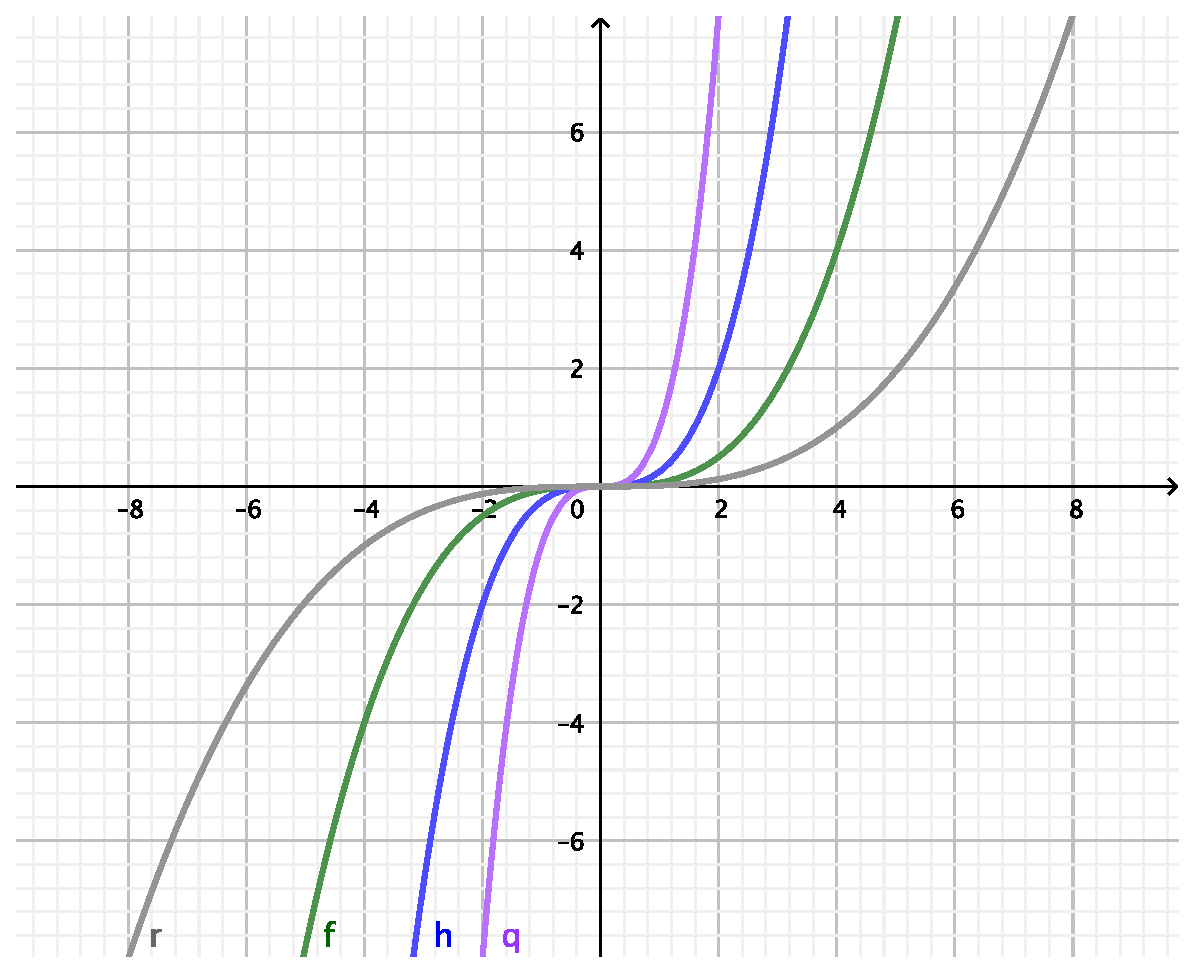
\includegraphics[height=12\baselineskip]{kap3/BundelFunktionenscharen.eps}
\end{minipage}

\subsection{Beispiel}

$f_{a}(x)= \dfrac{x^2-3ax}{x+a} \qquad \qquad D_{f} = \R \backslash \{ -a \}, \qquad a \in \R^+$

Sei $K_{a}$ der Graph der Funktion.


\subsubsection{Bestimmen Sie die Schnittpunkte von $K_{a}$ mit den Koordinatenachsen}

$f_{a}(0)=\dfrac{0}{x+a} = 0$

$\begin{array}{rcccl}
	\Rightarrow f_{a}(x)=0 & \Leftrightarrow & x^2-3x & = & 0 \\
	&\Leftrightarrow & x(x-3a) & = & 0 \\
	&\Leftrightarrow & x=0 & \lor & x  =  3a  \\
\end{array}$

Es ergeben sich die Punkte $P_{1}(0|0)$ und $P_{2}(3a|0)$

\subsubsection{Bestimmen Sie die Asymptoten von $K_{a}$}

$\begin{array}{rccccccl}
	 \Rightarrow & (x^2 & -3ax & +0) & : & (x+a) &=& x - 4a +\dfrac{4a^2}{x+a} \\ \\
	& -(x^2 & +ax) & & & & & \\ \\
	& & -4ax & +0 & & & & \\ \\
	& & -(-4ax & -4a^2) & & & & \\ \\
	& & & 4a^2 & & & & \\ \\
\end{array}$

Man erhält die schiefe Asymptote $y=x-4a$

Es liegt eine nicht hebbare Definitionslücke bei $-a$ vor, daraus ergibt sich eine vertikale Asymptote $\Rightarrow x=-a$


\subsubsection{Zeigen Sie $f''_{a}(x) = \frac{8a^2}{(x+a)^3}$}

$\begin{array}{rcl}
	f'_{a}(x) &=& \dfrac{(2x-3a)(x+a) - (x^2-3ax)(1)}{(x+a)^2} \\
	&=& \dfrac{2x^2+2ax-3ax-3a^2-x^2-3ax}{x^2+2ax+a^2}\\
	&=& \dfrac{x^2+2ax-3a^2}{(x+a)^2}  \\ \\
	f''_{a}(x) &=& \dfrac{(\textcolor{red}{2x+2a})(x^2+2ax+a^2) - (x^2-2ax-3a^2)(2(\textcolor{red}{x+a}) ) }{(x+a)^{\textcolor{red}{4}}}  \\
	&=& \dfrac{2x^2+4ax+2a^2-2x^2+4ax+6a^2}{(x+a)^3}\\
	&=& \dfrac{8a^2}{(x+a)^3}
\end{array}$

\subsubsection{Weisen Sie nach, dass $K_{a}$ genau einen Hochpunkt und genau einen Tiefpunkt besitzt. Geben Sie die Koordinaten dieser Punkte in Abhängigkeit von $a$ an und erstellen Sie eine Monotonietabelle der Funktionen $f_{a}$}

Notwendige Bedingung für Extremstellen: $\Rightarrow f'(x)=0$

$\Leftrightarrow x^2+2ax-3a^2 = 0 \qquad \qquad D= \R \backslash\{ -a \}$

$\Rightarrow \Delta = 4a^2 +12a^2 = 16a^2$

$\Leftrightarrow x_{1}=a \quad \lor \quad x_{2}=-3a \qquad \qquad L=\{a;-3a\}$

$\Rightarrow f(a)=\dfrac{a^2-3a^2}{2a} = -a$

$\Rightarrow f(-3a)= \dfrac{9a^2+9a^2}{-2a} = -9a$

Es ergeben sich somit die Extremstellen $H(-3a|-9a)$ und $T(a|-a)$. Bevor man mit der Monotonietabelle beginnt, muss die Polstelle untersucht werden.

$$\lim\limits_{x \rightarrow {-a^+}}{f_{a}} = \lim\limits_{x \rightarrow {-a^+}}{\dfrac{x^2-3ax}{x+a}} =\lim\limits_{h \rightarrow {0}}{\dfrac{(-a+h)^2 -3a(-a+h)}{(-a+h)+a}} = \lim\limits_{h \rightarrow {0}}{\dfrac{h^2-5ah+4a^2}{h}} = + \infty$$
$$\lim\limits_{x \rightarrow {-a^-}}{f_{a}} = \lim\limits_{x \rightarrow {-a^-}}{\dfrac{x^2-3ax}{x+a}} =\lim\limits_{h \rightarrow {0}}{\dfrac{(-a-h)^2 -3a(-a-h)}{(-a-h)+a}} = \lim\limits_{h \rightarrow {0}}{\dfrac{h^2+5ah+4a^2}{-h}} = - \infty$$
Jetzt kann die Monotonietabelle erstellt werden:

\begin{tikzpicture}
	\tikzset{arrow style/.style = {blue,->,> = latex',
	shorten > = 6pt,
	shorten < = 6pt}}
	\tkzTabInit{$x$ /1, $ x^2-2ax-3a $ /1.2, $(x+a)^2 $ /1.2, $f_{a}'(x)$ /1.2, $f_{a}(x)$ /3}{$-\infty$ ,$-3a$ , $-a$, $a$ ,$+\infty$}
	\tkzTabLine{{},+,z,-,t,-,z,+,}
	\tkzTabLine{{},+,t,+,d,+,t,+,}
	\tkzTabLine{{},+,z,-,d,-,z,+,}
	\tkzTabVar{ - / $-\infty$ , + / $H(-3a|-9a)$ / , -D+ / $-\infty$/$+\infty$  , - / $T(a|-a)$ , + / $+\infty$ }
\end{tikzpicture}

\subsubsection{Zeigen Sie, dass es genau einen Punkt gibt, durch den alle Graphen $Ka$ gehen.}

Diesen Punkt haben wir schon per "Zufall" herausgefunden, da wir eine Nullstelle gefunden haben, die nicht von $a$ abhängt. Wenn man diesen aber nicht gefunden hat, geht man diesen Lösungsweg:\\\\

$\begin{array}{rcccccl}
	\Rightarrow & f_{1}=f_{2} & \Leftrightarrow & \dfrac{x^2-3x}{x+1} & = & \dfrac{x^2-6x}{x+2} & \qquad \qquad D=\R \backslash \{-1;-2\} \\ \\
	&&\Leftrightarrow& \dfrac{x-3}{x+1} &=& \dfrac{x-6}{x+2}&  \\\\
	&&\Leftrightarrow& -x & = & -5x &\\ \\
	&&\Leftrightarrow& x &=& 0 & \qquad \qquad L=\{ 0 \} \\
\end{array}$

\subsubsection{Bestimmen Sie $a\in \R^+$ so, dass der Graph $K_{a}$ durch den Punkt $P(5|\frac{5}{3})$ verläuft}

$\begin{array}{rcccccl}
	\Rightarrow & f_{a}(5) = \dfrac{5}{3} & \Leftrightarrow & \dfrac{5^2-15a}{5+a} &=& \dfrac{5}{3} & \qquad \qquad D=\R \backslash \{-5\} \\\\
	&&\Leftrightarrow & 15-9a &=& 5+a &\\\\
	&&\Leftrightarrow & a&=&1&\qquad \qquad L=\{1\}\\\\
\end{array}$

\subsubsection{ Berechnen Sie die Schnittpunkte von $K_{1}$ mit der Geraden $j(x) =-15x -4$ }

$\begin{array}{rcccl}
	\Rightarrow  f_{1}(x) & = & \dfrac{x^2-3x}{x+1} &=& -15x-4 \quad = \quad y\\\\
	&\Leftrightarrow & x^2-3x &=& -15x^2-19x-4\\\\
	&\Leftrightarrow & 4x^2+4x+1 &=& 0\\\\
	\Delta = 0 & \Rightarrow &x &=& -\dfrac{1}{2}
\end{array}$

$\Rightarrow f_{1}(-\dfrac{1}{2}) = \dfrac{(\frac{1}{2})^2 -3\cdot (\frac{1}{2})}{-\frac{1}{2}+1} = \dfrac{7}{2}$

Es existiert genau ein Schnittpunkt von $K_{1}$ mit der Geraden $j$: $P_{K_{1}j}(-\frac{1}{2}|\frac{7}{2})$

\subsubsection{ Vom Punkt $A(0|-4)$ wird die Tangente an $K_{1}$ gelegt. Bestimmen Sie eine Gleichung der Tangente und die Koordinaten des Berührpunktes }

Sei $B(x_{0}|f_(x_{0}))$, dann lautet die Tangentengleichung:

$\begin{array}{rccl}
	\Rightarrow & T_{x_{0}}(x) &=& f'(x_{0}) \cdot (x-x_{0}) +f(x_{0}) \\ \\
	&&=& \dfrac{x_{0}^2 +2x_{0}-3}{(x_{0}+1)^2} \cdot (x-x_{0}) + \dfrac{x_{0}^2 -3x_{0}}{x_{0}+1}
\end{array}$

Jetzt werden die Koordinaten des Punktes $A(0|-4)$, durch den die Tangente auch noch geht, eingesetzt.

$\begin{array}{rcccccl}
	\Rightarrow & T_{x_{0}}(0) &=& -4 & = & \dfrac{x_{0}^2 +2x_{0}-3}{(x_{0}+1)^2} \cdot (-x_{0}) + \dfrac{x_{0}^2 -3x_{0}}{x_{0}+1} &\qquad \qquad D=\R \backslash \{ -1\}\\\\
	\Leftrightarrow &&& -4 (x_{0}+1)^2 &=& (x_{0}^2+2x_{0}-3)(-x_{0})+(x_{0}^2-3x_{0})(x_{0}+1) & \\\\
	\Leftrightarrow &&& -4x_{0}^2-8x_{0}-4 &=& -x_{0}^3-2x_{0}^2+3x_{0}+x_{0}^3+x_{0}^2-3x_{0}^2-3x_{0}& \\\\
	\Leftrightarrow &&& 4x_{0}^2+8x_{0}+4 &=& 4x_{0}^2&\\\\
	\Leftrightarrow &&& x_{0} &=& -\dfrac{1}{2}&\qquad \qquad L= \left \{ -\dfrac{1}{2} \right \}
\end{array}$

Nun werden die Koordinaten des Berührpunktes mit der Ursprünglichen Funktion $f$ durch einsetzen errechnet.

$$\Rightarrow f_{1} \left (-\dfrac{1}{2}\right ) =  \dfrac{\left (-\frac{1}{2}\right ) ^2-3\cdot - \frac{1}{2}}{-\frac{1}{2}+1} = \dfrac{7}{2} $$

$$\Rightarrow B \left (-\dfrac{1}{2}| \dfrac{7}{2} \right )$$

Da es sich um eine Tangente handelt, muss nun die Steigung am Berührpunkt errechnet werden, um die Tangentengleichung bestimmen zu können.

$$\Rightarrow f_{1}' \left (-\dfrac{1}{2} \right ) = \dfrac{\left (-\frac{1}{2} \right )^2 +2\left (-\frac{1}{2} \right ) -3 }{\left (-\frac{1}{2} \right )^2}  = -15$$

Die Tangentengleichung lautet somit:
$$t(x) = -15x-4\qquad \quad \text{mit} \quad D_{t}=\R$$


\end{document}
